
\documentclass[letterpaper,twocolumn,10pt]{article}
\usepackage{usenix2019_v3}

% to be able to draw some self-contained figs
\usepackage{tikz}
\usepackage{amsmath}
\usepackage{pgfplots}

% inlined bib file
\usepackage{filecontents}

\begin{document}
%-------------------------------------------------------------------------------

%don't want date printed
\date{}

% make title bold and 14 pt font (Latex default is non-bold, 16 pt)
\title{\Large \bf General Matrix Multiplication (GEMM) with OpenMP}

%for single author (just remove % characters)
\author{
{\rm Robert Geil}\\
University of California, Los Angeles
} % end author

\maketitle

%-------------------------------------------------------------------------------
\begin{abstract}
%-------------------------------------------------------------------------------
General Matrix Multiplication (GEMM) is an important problem type in many fields
of computer science and is therefore a good candidate for optimization and
parallelization. In this lab, we utilized cacheing and parallel programming with
OpenMP to speedup the multiplication of large matricies as compared to a na\"{i}ve 
approach, reaching roughly 110 Gigaflops at peak
\end{abstract}


%-------------------------------------------------------------------------------
\section{Introduction}
%-------------------------------------------------------------------------------

Matrix multiplication is a problem that arises in many areas of computer science,
from image processing to AI. As such, by optimizing this one problem, many slow
processes can be sped up and take advantage of the compute resources in the
many core era. To that end, we would like to apply both parallelism through
OpenMP as well as improve cache performance by limiting cache misses. To achieve
these goals, we will use OpenMP's preprocessor statements for parallelism, and
use loop permutations to improve cache hit rates.

%-------------------------------------------------------------------------------
\section{Machine Specifications}
%-------------------------------------------------------------------------------

The machine for which the code was optimized is an Amazon Web Services (AWS)
\textit{m5.2xlarge} virtual machine. This machine has 4 virtual CPUs, each of
which supports 2 threads via Intel's Hyperthreading technology. The processor is
clocked at 3.1 GHz, and contains 32 Kb L1, 1024 Kb L2 and 33792 Kb L3 cache.

%-------------------------------------------------------------------------------
\section{Solution Approach}
%-------------------------------------------------------------------------------
For this problem, we took two approaches. First was a \textit{parallel} approach, where
we only used loop reordering and OpenMP to improve the performance of the code.
In the other approach, \textit{parallel blocked}, we both used OpenMP for parallelization
and used a technique called \textit{loop tiling} to extract more performance from
the cache.
\subsection{OpenMP}
To integrate OpenMP into the solution, we used the preprocessor directives portion
of OpenMP. The one most heavily utilized was the parallel for loop, as seen below
\begin{verbatim}
#pragma parallel for private(j, k)
for(int i = 0; ...){
\end{verbatim}
This, placed just outside the outermost for loop of the multiplication split the
work among a number of threads, each taking a portion of the multiplication.
Here private variables were used to prevent the threads from overwriting each
other's $j$ and $k$ variables as they proceeded through the inner loops. In addition,
for the \textit{parallel blocked} implemention, additional variables for the blocks
were added to the private list, as well as a \textit{schedule(static, 32)} which was
found to improve performance by scheduling larger blocks to work at the same time.
\subsection{Loop Ordering}
The na\"{i}ve approach to matrix multiplication uses a triple for loop first iterating
over $i$, then $j$ and finally $k$
\begin{verbatim}
for(int i = 0; i<I; i++){
  for(int j = 0; j<J; j++){
    for(int k = 0; k<K; k++){
      c[i][j] = a[i][k]*b[k][j];
    }
  }
}
\end{verbatim}
However, because of how matrices are laid out in memory, this turns out to be a 
quite inefficient approach. Since arrays in C/C++ are stored in row-major order,
increasing k frequently as part of the innermost loop means that matrix $b$ cannot
be effectively cached, as each time a whole new row must be read from main memory.
To improve on this, we can reorder the loops without changing the semantics of the
program as follows
\begin{verbatim}
  for(int i = 0; i<I; i++){
    for(int k = 0; k<K; k++){
      for(int j = 0; j<J; j++){
        c[i][j] = a[i][k]*b[k][j];
      }
    }
  }
  \end{verbatim}
With this reordering, we see that the value read from a can be cached for $J$ 
iterations, while the values read from b and stored to c exhibit spatial
locality, as they are being read linearly from memory.
\subsection{Loop Tiling}
With a traditional matrix multiplication of matricies, lots of cache lines are
crossed as the multiplication proceeds through the matrix. To improve this
performance, we can use a technique called \textit{loop tiling}, where the
matrix is processed in $b$x$b$ blocks, so as to improve the temporal locality.
The following code was used to tile the matrix multiplication for our
\textit{parallel-blocked} implementation
%\begin{minipage}{\linewidth}
\begin{verbatim}
for (int i = 0; i < kI; i += BLOCK_SIZE){
  for (k = 0; k < kK; k += BLOCK_SIZE){
    for (ii = i; ii < i + BLOCK_SIZE; ++ii){
      for (ik = k; ik < k + BLOCK_SIZE; ++ik){
        for (j = 0; j < kJ; j++){
          c[ii][j] += a[ii][ik] * b[ik][j];
        }
      }
    }
  }
}
\end{verbatim}
%\end{minipage}
As can be seen from the code, the same number of matrix multiplication operations
are being computed, but the elements within a block are repeatedly used, before
jumping to the next block, helping improve cache rates.
%-------------------------------------------------------------------------------
\section{Results}
%-------------------------------------------------------------------------------
\begin{figure}
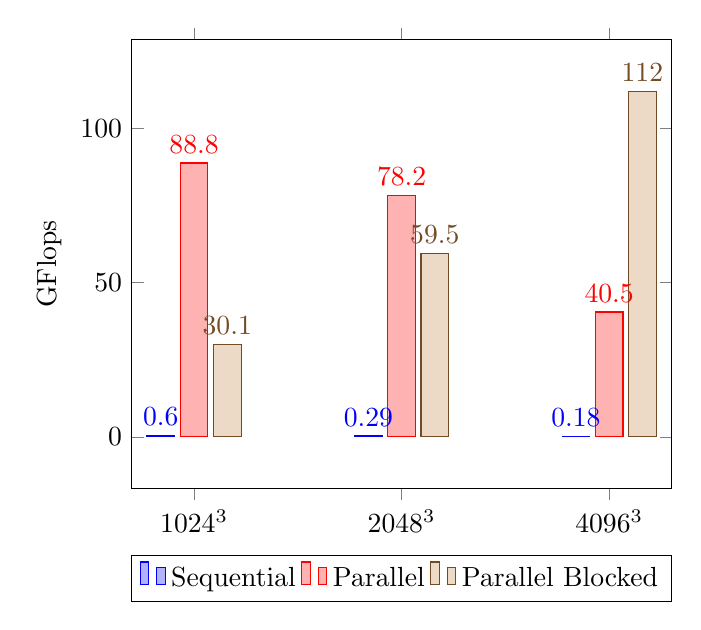
\begin{tikzpicture}
  \begin{axis}[
      ybar,
      enlargelimits=0.15,
      legend style={at={(0.5,-0.15)},
        anchor=north,legend columns=-1},
      ylabel={GFlops},
      symbolic x coords={$1024^3$,$2048^3$,$4096^3$},
      xtick=data,
      nodes near coords,
      nodes near coords align={vertical},
      ]
      \addplot coordinates {($1024^3$,0.60) ($2048^3$,0.29) ($4096^3$,0.18)};
      \addplot coordinates {($1024^3$,88.8) ($2048^3$,78.2) ($4096^3$,40.5)};
      \addplot coordinates {($1024^3$,30.1) ($2048^3$,59.5) ($4096^3$,112)};
  \legend{Sequential,Parallel,Parallel Blocked}
  \end{axis}
  \end{tikzpicture}
  \caption{\label{fig:comp} Performance results for various problem sizes}
\end{figure}
As can be seen in figure~\ref{fig:comp}, both the parallel and parallel-blocked
versions have a huge impact on performance, improving in the worst case by about 50 times,
and in the best case over 600 times as compared to sequential programming. One
consideration is how the performance of the blocked vs. unblocked versions change
as a factor of problem size. As seen in figure~\ref{fig:comp}, the performance of
the regular parallel version decreases, going from roughly 90GFlops to about 40GFlops
when going from $1024^3$ to $4096^3$. This occurs because the cache performance worsens
as the rows of the matrix become longer. By comparison, the \textit{blocked parallel}
performance improves as the problem size increases, as the improvements of the
cache hit rate make up for the increased number of jumps and register values
required for the further nested \textbf{for} loops.
\subsection{OMP Blocked Performance}
We attempted to optimize the \textit{blocked parallel} solution for the $4096^3$
size problem. As such, we set both the block size and the static subdivision
among threads to dynamic values. After sampling performance, we found that a block
size of 32 and a static workload size of 32 was most efficient. The block size
let more data fit into cache, while the workload size helped reduce the need for
thread scheduling, which occurred when
\begin{verbatim}
#pragma omp ... schedule(static, 32)
\end{verbatim}
was not there.
\begin{figure}
  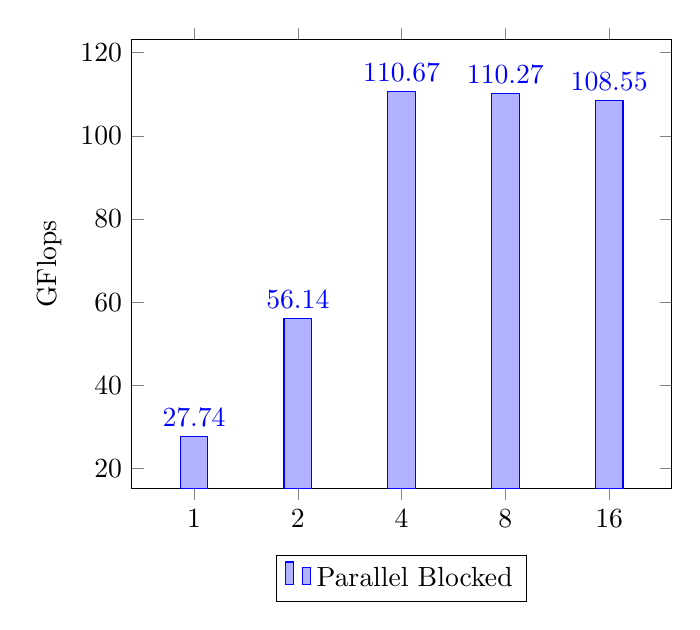
\begin{tikzpicture}
    \begin{axis}[
        ybar,
        enlargelimits=0.15,
        legend style={at={(0.5,-0.15)},
          anchor=north,legend columns=-1},
        ylabel={GFlops},
        symbolic x coords={1,2,4,8,16},
        xtick=data,
        nodes near coords,
        nodes near coords align={vertical},
        ]
        \addplot coordinates {(1,27.74) (2,56.14) (4,110.67) (8,110.27) (16,108.55)};
    \legend{Parallel Blocked}
    \end{axis}
    \end{tikzpicture}
    \caption{\label{fig:threads} Performance of \textit{parallel blocked} with 
    different numbers of threads on $4096^3$ matrices}
  \end{figure}
As can be seen in figure~\ref{fig:threads}, there is a direct impact on the number
of threads made available to the program and the performance in terms of GFlops.
Increasing from 1 to 2 to 4 threads results in a near doubling of performance each
time. However, increasing to 8 threads actually results negligable a performance loss.
This is because while the computer has 8 threads through Virtualization, the physical
CPUs and cache are still only that of 4 cores. Therefore, increasing to 8 threads to
attempt to take advantage of the additional virtual threads only introduces scheduling
overhead. The same can be seen by increasing to 16 threads. This simply adds more
context switching and doesn't improve the performance of the whole system.
\section{Difficulties}
Some difficulties I encountered included workspace setup. It was difficult to get
started programming remotely on the AWS machine, and I ended up using VSCode's
remote workspace extension, letting me work via SSH in an IDE, so rapid testing could
be performed. Another challenge I faced and was unable to resolve was profiling
the cache. I attempted to install \textit{valgrind} and use their cache profiler,
but there was an issue where \textit{valgrind} encountered an illegal instruction
in the base code provided, when passing arrays to the functions. As a result I was
not able to perform this profiling and get a finer-grain parallelism along the cache lines.
\end{document}
%%%%%%%%%%%%%%%%%%%%%%%%%%%%%%%%%%%%%%%%%%%%%%%%%%%%%%%%%%%%%%%%%%%%%%%%%%%%%%%%